\section{Summary of Time Marching Solution}\label{summary-of-time-marching-solution}

EnergyPlus models building performance over time spans of days to years using a time marching method based on \emph{timesteps}. This section provides more information on issues related to timestep formulation.

\subsection{Summary of Timestep Model Formulation}\label{summary-of-timestep-model-formulation}

An EnergyPlus simulation covers a certain period of time, such as a day or a year, that is broken down into a series of discrete bins of time that are referred to as \emph{timesteps}. The program marches through time by recalculating model equations at each timestep. The figure below diagrams some of these basic concepts.

\begin{figure}[hbtp] % fig 9
\centering
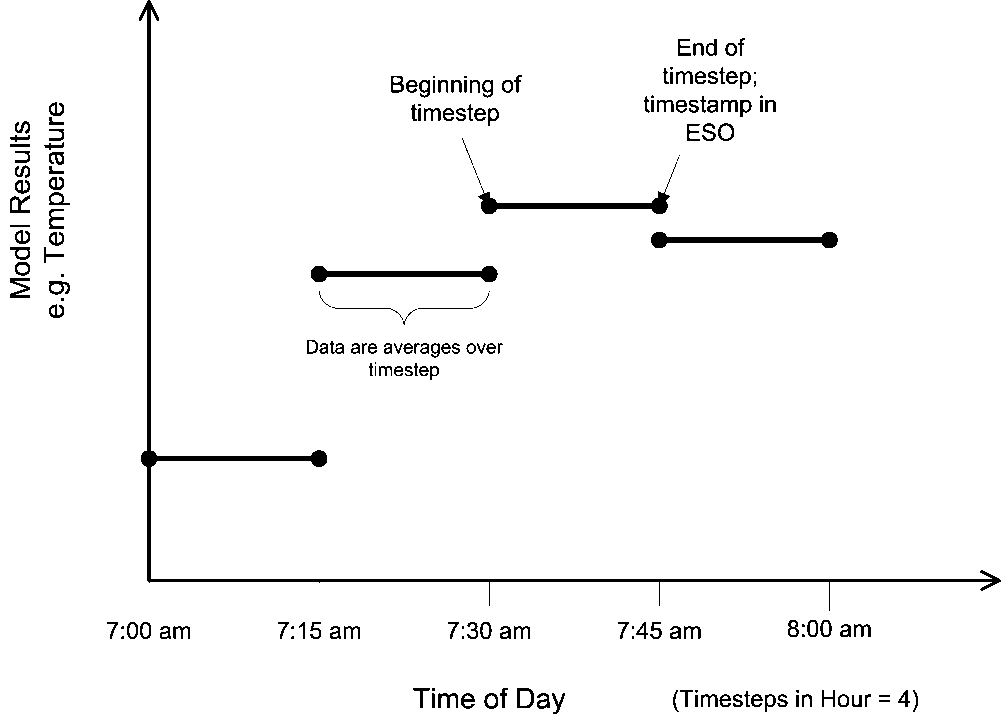
\includegraphics[width=0.9\textwidth, height=0.9\textheight, keepaspectratio=true]{media/image141.png}
\caption{Diagram of TimeStep Formulation \protect \label{fig:diagram-of-timestep-formulation}}
\end{figure}

Most models in EnergyPlus are quasi-steady energy balance equations used to predict the conditions present during each timestep. Various input data and boundary conditions for the models are time-varying and a ``staircase'' approach is used where such values are determined for a particular timestep and then essentially held constant over the entire timestep. Predictions for state variables, such as temperature, are averages over the timestep. Predictions for summed variables, such as energy use, are simple totals over the timestep.

EnergyPlus produces time-series results for selected output variables at selected frequencies. The time values associated with the time-series data, or timestamps, are output for the end of the timestep, but the values of the variables are for the entire bin of time prior to the timestamp. When data are reported at coarser frequencies such as hourly, then the results are averages or simple totals for all the timesteps that are contained within the larger bin of time.

To simplify solutions that would otherwise need to be simultaneous, models sometimes use data that are ``lagged'' which means that the values used in the calculations for the current timestep are actually results from the previous timestep. Many models just use the most current results available and so may use lagged data for a first iteration, but then use current data that are not lagged for subsequent iterations.

\subsection{Zone Update Method}\label{zone-update-method}

A zone is not necessarily a single room but is usually defined as a region of the building or a collection of rooms subject to the same type of thermal control and having similar internal load profiles that, subsequently, can be grouped together. Zones can interact with each other thermally through adjacent surfaces and by intermixing of zone air. In EnergyPlus, the conditions in each zone are updated by Equation~\ref{eq:TztFromZoneAirEnergyBalance}, which uses previously calculated values of the zone conditions. This means that EnergyPlus does not have to iterate to find a self-consistent solution of the updated zone conditions. However, because heat transfer through each zone's surfaces and interzone mixing of air still occur, the new space temperatures must be computed at the same simulation time and on the same time step in all zones, even though conditions in one zone may be changing much more rapidly than conditions in the other zones. We have previously documented the method used to update the zone temperature at each time step. This method, called the predictor corrector method, has proved to be satisfactory over a wide range of conditions.

\subsection{Variable Timestep}\label{variable-timestep}

The need for a variable timestep in EnergyPlus was identified during development of its predecessor IBLAST. Prior to the integration of the central plant simulation in IBLAST, a time step Dt for the zone temperature update of 0.25 hours (15 minutes) was found to give stable results without a large increase in computation time. The first step in integrating plant was to implement the detailed coil models and coil control strategies without actually adding the plant models themselves. This meant that the user had to specify the coil water inlet temperature and the maximum coil inlet water flow rate to run the simulation. The real life analogy would be a chiller of very large, though not infinite, capacity. The coil capacity was controlled by adjusting the water flow rate, but the effect of the plant on the chilled water temperature was eliminated. After implementation of this step, experience with the program showed that updating the zone temperatures on a fixed time step frequently resulted in instabilities unless a very short time step was used. However, as the time step got shorter the time required to execute the program got prohibitively high.

Clearly, an adaptive time step was required. This would shorten the time step to maintain stability of the zone air energy balance calculation when zone conditions were changing rapidly and expand it to speed computation when zone conditions were relatively unchanging. But, the adaptive time step could not be applied easily to the surface heat transfer calculations, even using interpolation methods to determine new temperature and flux histories. The problem of updating the zone temperature was resolved by using a two-time-step approach in which the zone air temperature is updated using an adaptive time step that ensures stability. In this two time level scheme, the contributions to the zone loads from the surfaces, and user specified internal loads are updated at the default or user specified time step that is constant. This is often referred to as the ``zone'' time step. The contributions to the zone loads from HVAC system response, infiltration, and air mixing are updated at a second variable time step, referred to as the ``system'' time step. The system time step is limited to between one minute and the zone time step. The lower limit of the system time step can be increased to larger than one minute by the user with a System Convergence Limits object (which may be useful to decrease simulation run times at the expense of some accuracy).

The program's decision to adapt the time step is made by first using the usual zone time step and executing the full predictor-corrector calculations to find resulting zone temperatures. The maximum temperature change experienced by any zone in the model is determined. If this maximum zone temperature change is more than a preset limit of 0.3°C, then the simulation switches to using the shorter system time step. The number of system time steps (within a particular zone time step) is modeled from the results for the maximum zone temperature change (just obtained from the corrector) by assuming that temperature change is linear. The number of system time steps indicated by the temperatures is:

\begin{equation}
\left( {\frac{{Maximum{\kern 1pt} \;Zone\;Temperature\;Change}}{{Maximum\;Zone\;Temperature\;Difference\;\{ .3C\} }}} \right) + 1.0
\end{equation}

The limit for the number of system time steps is:

\begin{equation}
\left( {\frac{{Zone\;Time\;Step}}{{Minimum\;System\;Time\;Step}}} \right)
\end{equation}

EnergyPlus takes the smallest of these two, truncates them to a whole number and calculates a system time step as:

\begin{equation}
System\;Time\;Step = \left( {\frac{{Zone\;Time\;Step}}{{Number\;of\;System\;Time\;Steps}}} \right)
\end{equation}

The same length of time is used for all the system time steps within a particular zone time step, but the system time step length can vary between different zone time steps. Report variables that use the ``detailed'' frequency show results at the system time step time scale.

This approach can be justified because the internal loads and surface temperatures vary on a different and longer time scale than the system response and the zone air temperature.

When the simulation down-steps from using the zone time step to the system time step, linear interpolation is used to generate zone condition history terms:

\begin{equation}
\begin{array}{l}
  T_z^{t-\delta t} \\
  T_z^{t-2\delta t} \\
  T_z^{t-3\delta t}
\end{array}
\end{equation}

for the system time steps using the history data for the zone time step. If two consecutive zone time steps both down-step to have the same number of system time steps, then the system time step history is preserved and used directly rather than being interpolated from zone time step history. The zone temperature update is made for each system time step using the same equation as for the zone time step except that the zone temperature history and time difference (\(\delta t\)) terms are for the system time step instead of for the zone time step.

\subsection{Simultaneous Solution of Plant/System Water Loop}\label{simultaneous-solution-of-plantsystem-water-loop}

Simultaneous solution of the system and plant operating parameters required that the temperature of the water entering the coils must be the same as the temperature leaving the chillers or boilers. In addition, the temperature of the return water from the coils must be equal to the chiller or boiler entering water temperature. In practice so long as the plant is not out of capacity the leaving water temperature from chillers and boilers is constant and equal to the design value. No iteration was required to match system and plant boundary conditions. However, if either the chiller or boiler plant was overloaded then the temperature of the water leaving the plant was not equal to the design value and the maximum output of the plant could change because of the off-design conditions. An iterative scheme using the secant method to predict successive updates to the plant leaving water conditions was therefore employed to solve for the water loop conditions with the plant operating at its maximum capacity. The simulation of the system and plant loops is described in greater detail in the later sections.

\subsection{References}\label{references-043}

Ceylan, H. T., and G. E. Myers. 1980. Long-time Solutions to Heat Conduction Transients with Time-Dependent Inputs. ASME Journal of Heat Transfer, Volume 102, No. 1, pp.~115-120.

Hittle, D. C. 1979. Calculating Building Heating and Cooling Loads Using the Frequency Response of Multilayered Slabs, Ph.D.~Thesis, University of Illinois, Urbana, IL.

Hittle, D. C., and R. Bishop. 1983. An Improved Root-Finding Procedure for Use in Calculating Transient Heat Flow Through Multilayered Slabs. International Journal of Heat and Mass Transfer, Vol. 26, No. 11, pp.~1685-1693.

Ouyang, K., and F. Haghighat. 1991. A Procedure for Calculating Thermal Response Factors of Multi-layered Walls--State Space Method. Building and Environment, Vol. 26, No. 2, pp.~173-177.

Seem, J. E. 1987. Modeling of Heat Transfer in Buildings, Ph.D.~Thesis, University of Wisconsin, Madison, WI.

Strand, R. K. 1995. Heat Source Transfer Functions and Their Application to Low Temperature Radiant Heating Systems, Ph.D.~Thesis, University of Illinois, Urbana, IL.

Taylor, R. D., C.O. Pedersen, L.K. Lawrie. 1990. \emph{Simultaneous Simulation of Buildings and Mechanical Systems in Heat Balance Based Energy Analysis Programs}, Proceedings of the 3rd International Conference on System Simulation in Buildings, Liege, Belgium, December 3-5, 1990.

Taylor, R.D., C.O. Pedersen, D.E. Fisher, R. J. Liesen, L.K. Lawrie. 1991. Impact of Simultaneous Simulation of Buildings and Mechanical Systems in Heat Balance Based Energy Analysis Programs on System Response and Control, Conference Proceedings IBPSA Building Simulation '91, Nice, France, August 20-22, 1991.
